%% body.tex
\section{系统设计}

\begin{frame}{系统总体架构}
    \footnotesize
    \begin{columns}
        \column{.40\textwidth}
        \begin{figure}
            \centering
            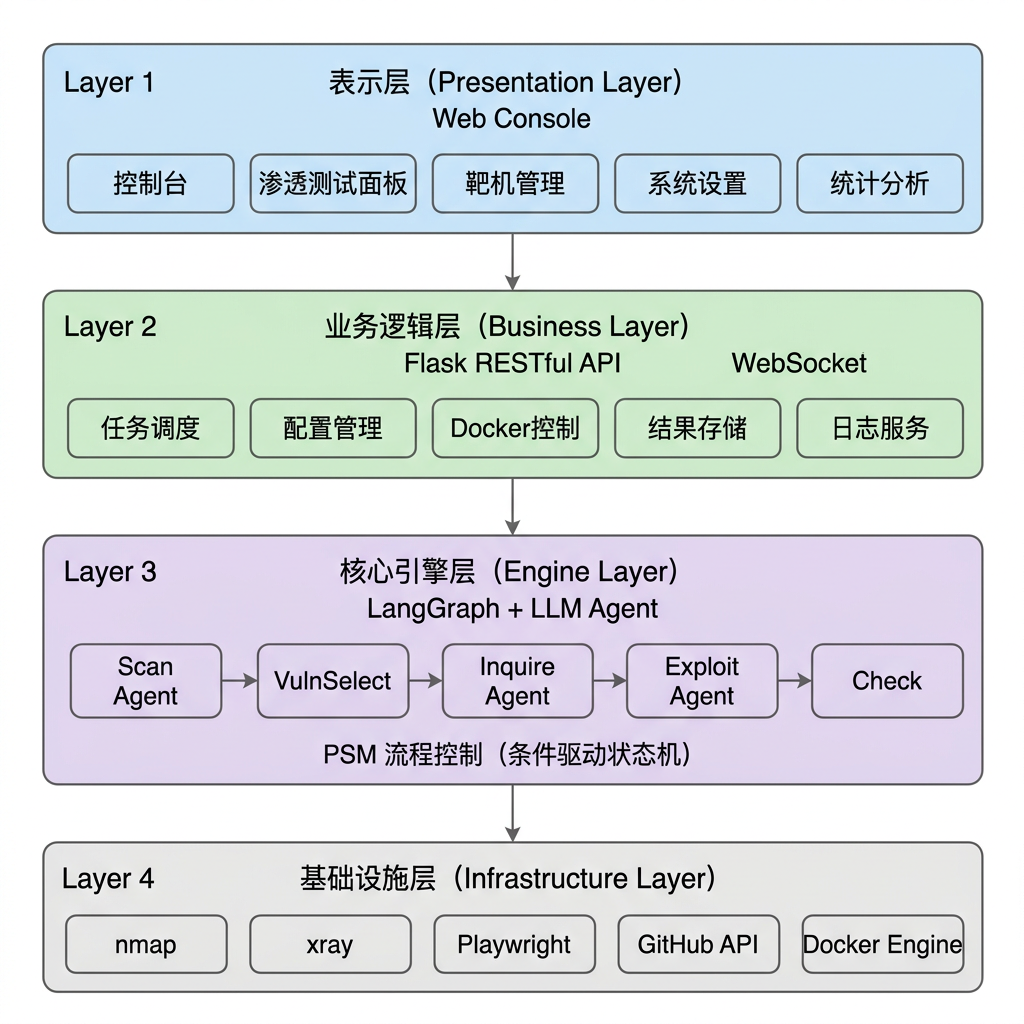
\includegraphics[width=\columnwidth,height=0.55\textheight,keepaspectratio]{contents/figure/arch.png}
            \caption{AutoPT+ 四层架构图}
        \end{figure}

        \column{.46\textwidth}
        \begin{block}{分层设计}
            \begin{itemize}
                \item \textbf{表示层}：Web Console（Flask + HTML）
                \item \textbf{业务逻辑层}：RESTful 接口、Docker 容器管理
                \item \textbf{核心引擎层}：LangGraph 状态机、Agent、VulnSelect / Check
                \item \textbf{基础设施层}：nmap · xray · Playwright · Docker Engine
            \end{itemize}
        \end{block}
    \end{columns}
\end{frame}

\section{改进一：PSM 流程控制}

\begin{frame}{提示词结构化与角色差异化}
    \footnotesize
    \begin{block}{统一 ReAct 基线模板}
        三个 Agent 共用 \_REACT\_HEADER / \_REACT\_FOOTER 骨架，FORMAT RULES 模块禁止 \texttt{<thinking>} 标签，将 Thought 限定为单句。
    \end{block}

    \begin{block}{三个 Agent 的角色边界}
        \begin{itemize}
            \item \textbf{Scan Agent}（SCAN ONLY, NO EXPLOITATION）：强制 nmap $\to$ xray $\to$ 结果的有序流程
            \item \textbf{Inquire Agent}（ONLY ReadHTML）：禁止执行命令，输出结构化多步 PoC（STEP N: 格式）
            \item \textbf{Exploit Agent}：明确 SUCCESS CRITERIA（/etc/passwd、uid=、phpinfo()），最多 8 次尝试
        \end{itemize}
    \end{block}
\end{frame}

\begin{frame}{Scan 阶段细化与提前终止机制}
    \footnotesize
    \begin{columns}
        \column{.48\textwidth}
        \begin{figure}
            \centering
            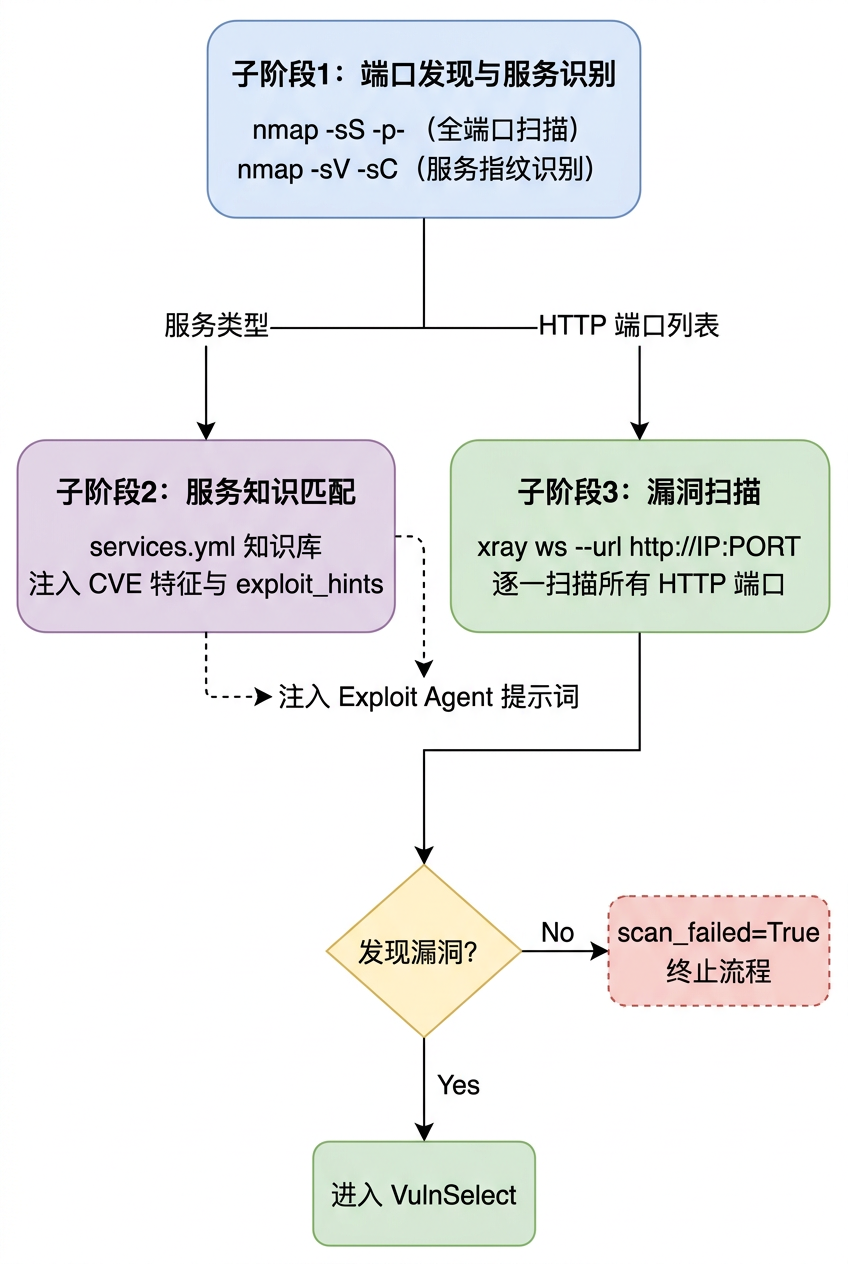
\includegraphics[width=\columnwidth,height=0.55\textheight,keepaspectratio]{contents/figure/scan.png}
            \caption{动态端口发现流程}
        \end{figure}

        \column{.48\textwidth}
        \begin{block}{四个子阶段}
            \begin{enumerate}
                \item \textbf{端口发现}：nmap -p- 全端口 + -sV -sC 服务识别
                \item \textbf{服务知识匹配}：services.yml 注入 CVE 特征与攻击线索（匹配率 85\% 精确 + 15\% 模糊 = 100\%）
                \item \textbf{漏洞扫描}：xray 对所有 HTTP 端口逐一扫描
                \item \textbf{结果评估}：parse\_vuln 解析为空则提前终止（try-except 防误判）；Exploit 调用次数 7.2$\to$4.8（\textbf{-33\%}）
            \end{enumerate}
        \end{block}
    \end{columns}
\end{frame}

\begin{frame}{上下文压缩与 Check 双层验证}
    \footnotesize
    \begin{columns}
        \column{.48\textwidth}
        \begin{block}{上下文压缩机制}
            \begin{itemize}
                \item \textbf{即时摘要}：关键 token 过滤（漏洞标识、服务指纹、错误信息），截断至 2000 字符
                \item \textbf{三层结构化组装}：Final Goal + 漏洞选择 + Scan 摘要
            \end{itemize}
        \end{block}
        \begin{block}{PoC 容错提取与 Check 双层验证}
            \begin{itemize}
                \item \textbf{PoC 四级容错}：Final Answer $\to$ agent\_log $\to$ ReadHTML 原始返回 $\to$ 日志回溯
                \item \textbf{匹配域缩小}：仅检查工具原始输出 raw\_outputs，排除模型推理文本
                \item \textbf{LLM 语义判断优先 + 正则通用匹配兜底} 双层校验
            \end{itemize}
        \end{block}

        \column{.48\textwidth}
        \begin{figure}
            \centering
            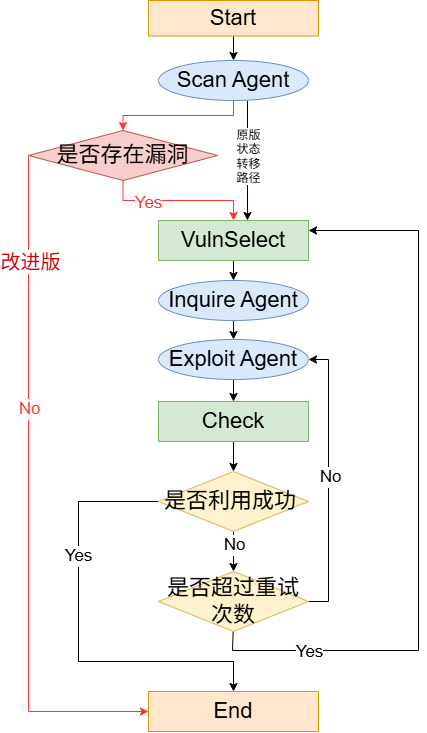
\includegraphics[width=\columnwidth,height=0.55\textheight,keepaspectratio]{contents/figure/psm.png}
            \caption{条件驱动的状态转移模型}
        \end{figure}
    \end{columns}
\end{frame}

\section{改进二：工具扩展与容错}

\begin{frame}{浏览器扩展工具与 RobustReActParser}
    \footnotesize
    \begin{columns}
        \column{.48\textwidth}
        \begin{block}{三个浏览器扩展工具}
            \begin{itemize}
                \item \texttt{fill\_element}：定位 input/textarea，清空后填入文本（安装向导、登录表单）
                \item \texttt{select\_option}：定位下拉框，按 value 或文本标签选择
                \item \texttt{wait\_for\_selector}：等待元素出现并可见，支持自定义超时
            \end{itemize}
        \end{block}

        \column{.48\textwidth}
        \begin{block}{RobustReActParser 多级容错}
            原版：格式偏差 $\to$ 直接抛异常终止循环 \\[0.5em]
            改进版通过降级策略（清洗思维链标签 $\to$ 标准解析 $\to$ 宽松正则 $\to$ Action 提取 $\to$ 模糊匹配 $\to$ 格式引导）将解析失败转为可恢复的中间状态。
        \end{block}
        \begin{block}{ReadHTML PoC 增强提取}
            匹配 GitHub vulhub 仓库时自动提取 README 中的 PoC 代码块，过滤环境搭建与 Docker 命令，仅返回利用相关命令。
        \end{block}
    \end{columns}
\end{frame}

\section{改进三：Web Console}

\begin{frame}{Web Console 图形化管理界面}
    \footnotesize
    \begin{columns}
        \column{.50\textwidth}
        \begin{block}{六个功能模块}
            \begin{itemize}
                \item \textbf{控制台}：系统状态总览、OWASP 分类统计
                \item \textbf{漏洞库}：20 个 CVE 展示，搜索/难度筛选
                \item \textbf{渗透测试面板}：一键发起，实时日志（1.5s 轮询）
                \item \textbf{靶机管理}：Docker 容器启/停/销毁监控
                \item \textbf{测试报告}：历史记录、成本/Token 多维分析
                \item \textbf{系统设置}：API Key、模型参数配置
            \end{itemize}
        \end{block}
        \begin{block}{技术选型}
            Flask RESTful · 原生 JavaScript SPA · HTTP 轮询 1.5s · textContent 防 XSS
        \end{block}

        \column{.46\textwidth}
        \begin{figure}
            \centering
            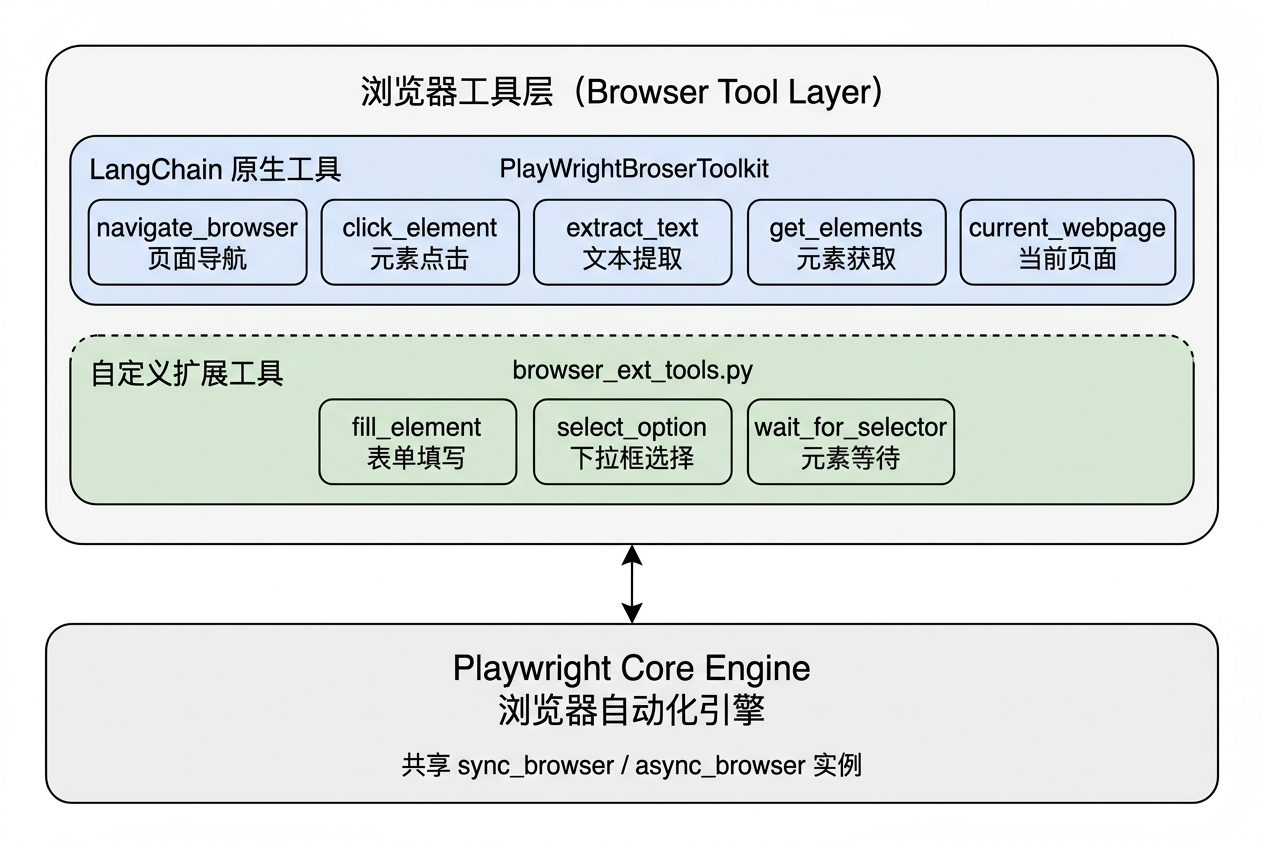
\includegraphics[width=\columnwidth,height=0.55\textheight,keepaspectratio]{contents/figure/browser.png}
            \caption{浏览器工具层架构}
        \end{figure}
    \end{columns}
\end{frame}

\section{实验与评估}

\begin{frame}{实验设置}
    \footnotesize
    \begin{block}{数据集}
        \begin{itemize}
            \item 20 个真实 CVE 漏洞（10 简单 + 10 复杂），涵盖 OWASP Top 10 全部类别
            \item 简单漏洞：1\textasciitilde2 个 HTTP 请求即可打通；复杂漏洞：需先走完安装向导，再对特定模块利用
        \end{itemize}
    \end{block}
    \begin{block}{模型与参数}
        \begin{itemize}
            \item 三个 LLM：GPT-4o、GPT-4o-mini、GPT-3.5-turbo，温度参数均固定为 0
            \item Scan Agent 最多 5 轮迭代，Inquire 3 轮，Exploit 12 轮，PSM 总递归深度上限 30 步
        \end{itemize}
    \end{block}
    \begin{block}{实验流程}
        \begin{itemize}
            \item 每漏洞每模型跑 5 次，共 \textbf{300 次}独立实验
            \item 每次实验后销毁重建 Docker 靶机，清空 Agent 上下文
            \item 原版 AutoPT 数据直接取自原论文\cite{Wu2024AutoPT}公开结果
        \end{itemize}
    \end{block}
\end{frame}

\begin{frame}{RQ1：模型差异分析}
    \footnotesize
    \begin{exampleblock}{核心结果}
        总体 24.67\% $\to$ \textbf{63.67\%（+39pp）} $\;|\;$ 简单 32\% $\to$ 76.67\% $\;|\;$ 复杂 17.33\% $\to$ 50.67\% $\;|\;$ 60 组 0\% $\to$ 仅 \textbf{3 组}
    \end{exampleblock}
    \begin{block}{三模型成功率排名}
        \textbf{GPT-4o-mini：74\%}（简单 90\%，复杂 58\%）$\gg$ GPT-4o：63\%（简单 76\%，复杂 50\%）$\gg$ GPT-3.5-turbo：54\%（简单 64\%，复杂 44\%）
    \end{block}
    \begin{alertblock}{弱模型"兜底"效应}
        GPT-3.5 原版 $\sim$7\% $\to$ \textbf{54\%}，增幅最大。合理的流程约束和提示词设计可在相当程度上补偿模型本身能力的不足。
    \end{alertblock}
    \begin{exampleblock}{现象}
        GPT-4o-mini 表现优于参数规模更大的 GPT-4o，与原论文\cite{Wu2024AutoPT}观察一致
    \end{exampleblock}
\end{frame}

\begin{frame}{RQ2：成本效益分析}
    \footnotesize
    \begin{columns}
        \column{.52\textwidth}
        \begin{table}
            \centering
            \scriptsize
            \begin{tabular}{@{}lccc@{}}
                \toprule
                \textbf{指标} & \textbf{原版} & \textbf{AutoPT+} & \textbf{人工} \\ \midrule
                总成本        & \$0.99 & \textbf{\$0.31} & $\sim$\$310 \\
                单次成本      & \$0.0099 & \textbf{\$0.003109} & — \\
                平均耗时/次   & 161.3s & \textbf{94.2s} & $\sim$15min \\
                总体成功率    & 36\%   & \textbf{74\%} & — \\ \bottomrule
            \end{tabular}
            \caption{成本效益对比（GPT-4o-mini，20 漏洞 $\times$ 5 次）}
        \end{table}

        \column{.44\textwidth}
        \begin{exampleblock}{结论}
            \begin{itemize}
                \item 费用降低 \textbf{69\%}
                \item 耗时缩短 \textbf{42\%}
                \item 成功率提升 \textbf{38pp}
            \end{itemize}
        \end{exampleblock}
        \begin{block}{原因}
            提前终止省去无效执行；上下文压缩减少 Token 用量
        \end{block}
    \end{columns}
\end{frame}


\begin{frame}{RQ3：改进效果评估}
    \footnotesize
    \begin{columns}
        \column{.52\textwidth}
        \begin{block}{三个改进方向效果}
            \textbf{PSM 流程}：提前终止省去无效执行，上下文压缩控制 Token 增长，提示词规范化减少越权命令 \\[0.3em]
            \textbf{工具扩展}：浏览器 + 容错解析 + PoC 增强，工具执行失败仅 \textbf{10.1\%}，错误的命令 29.4\%（4o-mini 最低 26.92\%） \\[0.3em]
            \textbf{Web Console}：提高实验过程一致性与结果可复核性，保障 300 组实验基础支撑
        \end{block}

        \column{.44\textwidth}
        \begin{table}
            \centering
            \scriptsize
            \begin{tabular}{@{}lcccc@{}}
                \toprule
                \textbf{失败原因} & \textbf{总体} & \textbf{3.5} & \textbf{4o} & \textbf{4o-mini} \\ \midrule
                提前放弃         & 33.0\%  & 32.6\% & 40.5\% & 23.1\% \\
                错误的命令       & 29.4\%  & 28.3\% & 32.4\% & 26.9\% \\
                上下文限制       & 22.9\%  & 19.6\% & 24.3\% & 26.9\% \\
                安全审查拦截     & 22.0\%  & 19.6\% & 18.9\% & \textbf{30.8\%} \\
                工具执行失败     & \textbf{10.1\%} & 13.0\% & 8.1\% & 7.7\% \\ \bottomrule
            \end{tabular}
            \caption{109 次失败的原因分布}
        \end{table}

        \begin{alertblock}{主要瓶颈}
            提前放弃（33\%）——重试策略不区分失败类型；安全审查拦截（22\%）——GPT-4o-mini 达 30.77\%
        \end{alertblock}
    \end{columns}
\end{frame}
